
\section{Metodology}

\subsection{Data acquiring}

The process of acquiring data was performed using satellite imagery provided by Landsat 7 satellite. In this process were downloaded 1362 satellite images, covering the department of Nariño, from years 1999 to 2015. To cover the whole department was necessary download satellite imagery with the next paths and rows: (009,059), (009,060), (010,058), (010,059), (011,059)

Also, in the data acquiring was used the biomass map build by  \cite{baccini2008afirst} for years 2000 to 2003.

\subsection{Preprocessing}

In this step, the imagery acquired was reprojected, because five images are in different coordinate systems (EPSG:32618 and EPSG:32617)  and were reprojected to the EPSG:3857 system. As well as the images were cut to cover the department of Nariño, as is shown in the figure~\ref{fig:Recortar imágenes}

\begin{figure}
  \centering
  \subfigure[Department of Narino satellite imagery]{\label{Imágenes Satélitales Nariño} 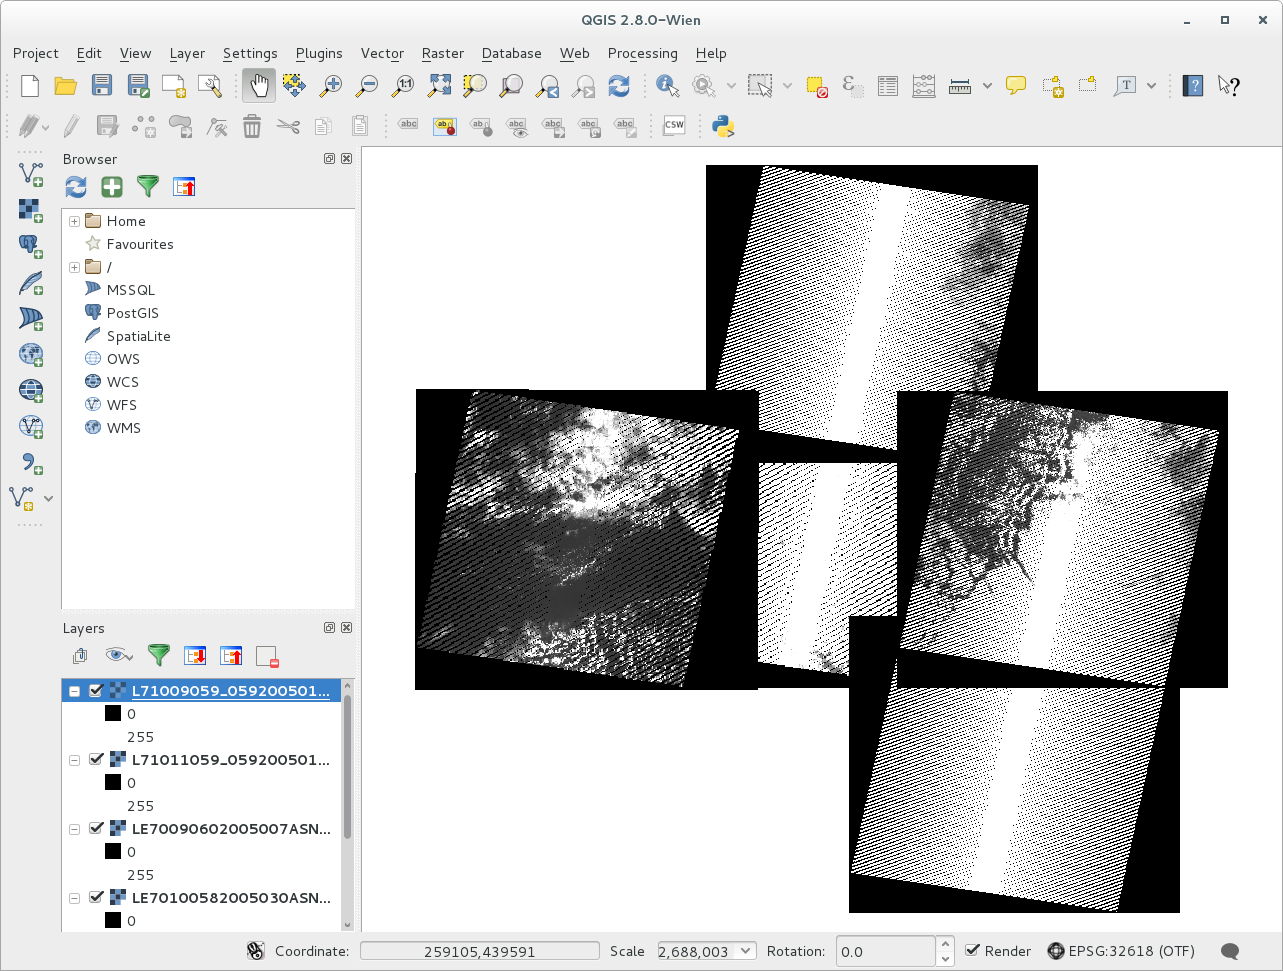
\includegraphics[width= 7cm]{cut1.png}}
  \vfill
  \subfigure[Department of Narino cut images]{\label{Imágenes recortadas de Nariño}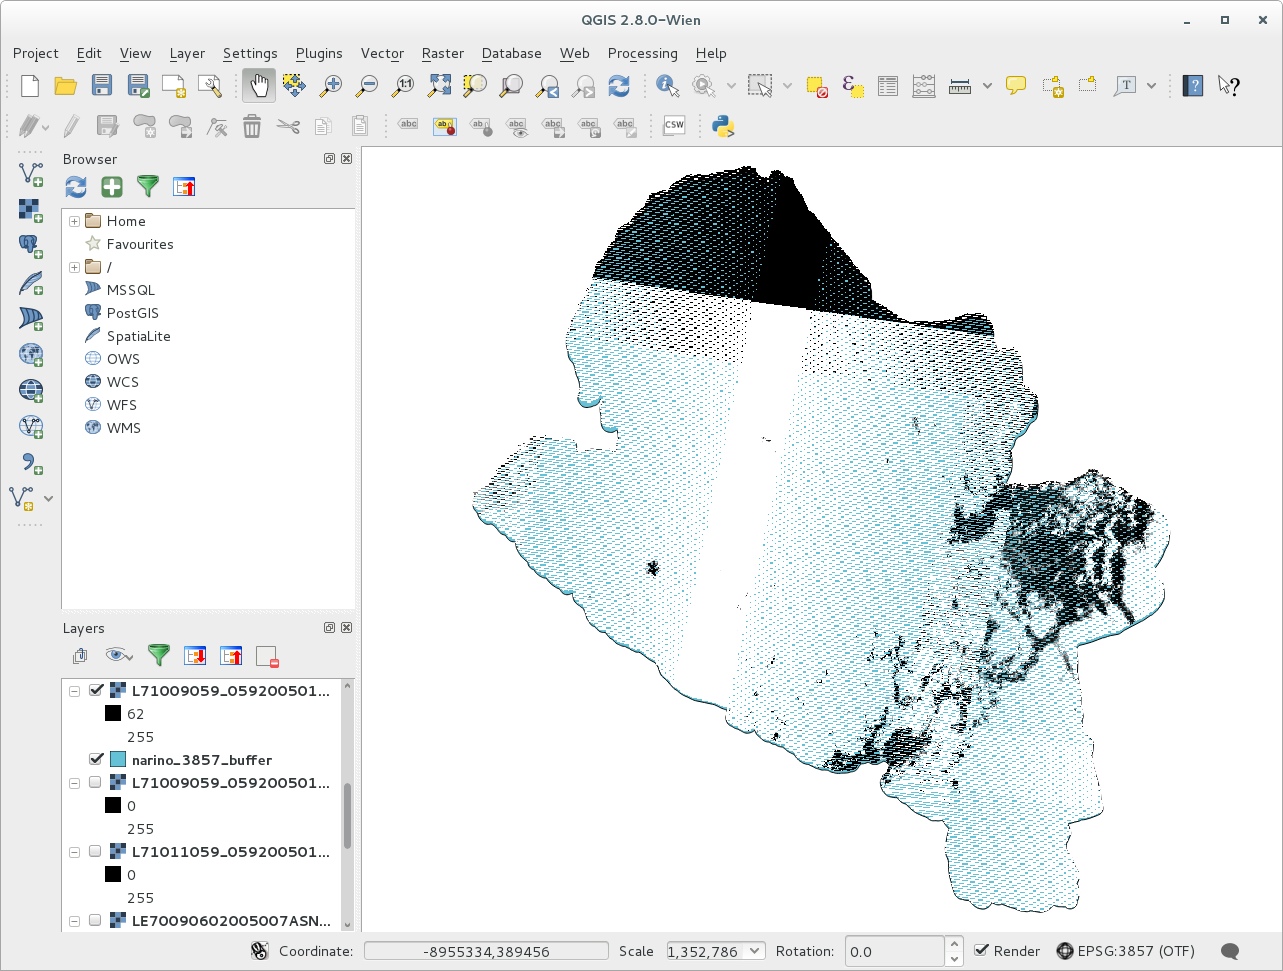
\includegraphics[width= 7cm]{cut2.png}}
  \caption{Preprocessing}
  \label{fig:Recortar imágenes}
\end{figure}

Similarly, this process was applied to biomass map as is shown in the figure~\ref{fig:mapaNarino}

\begin{figure}
  \centering
  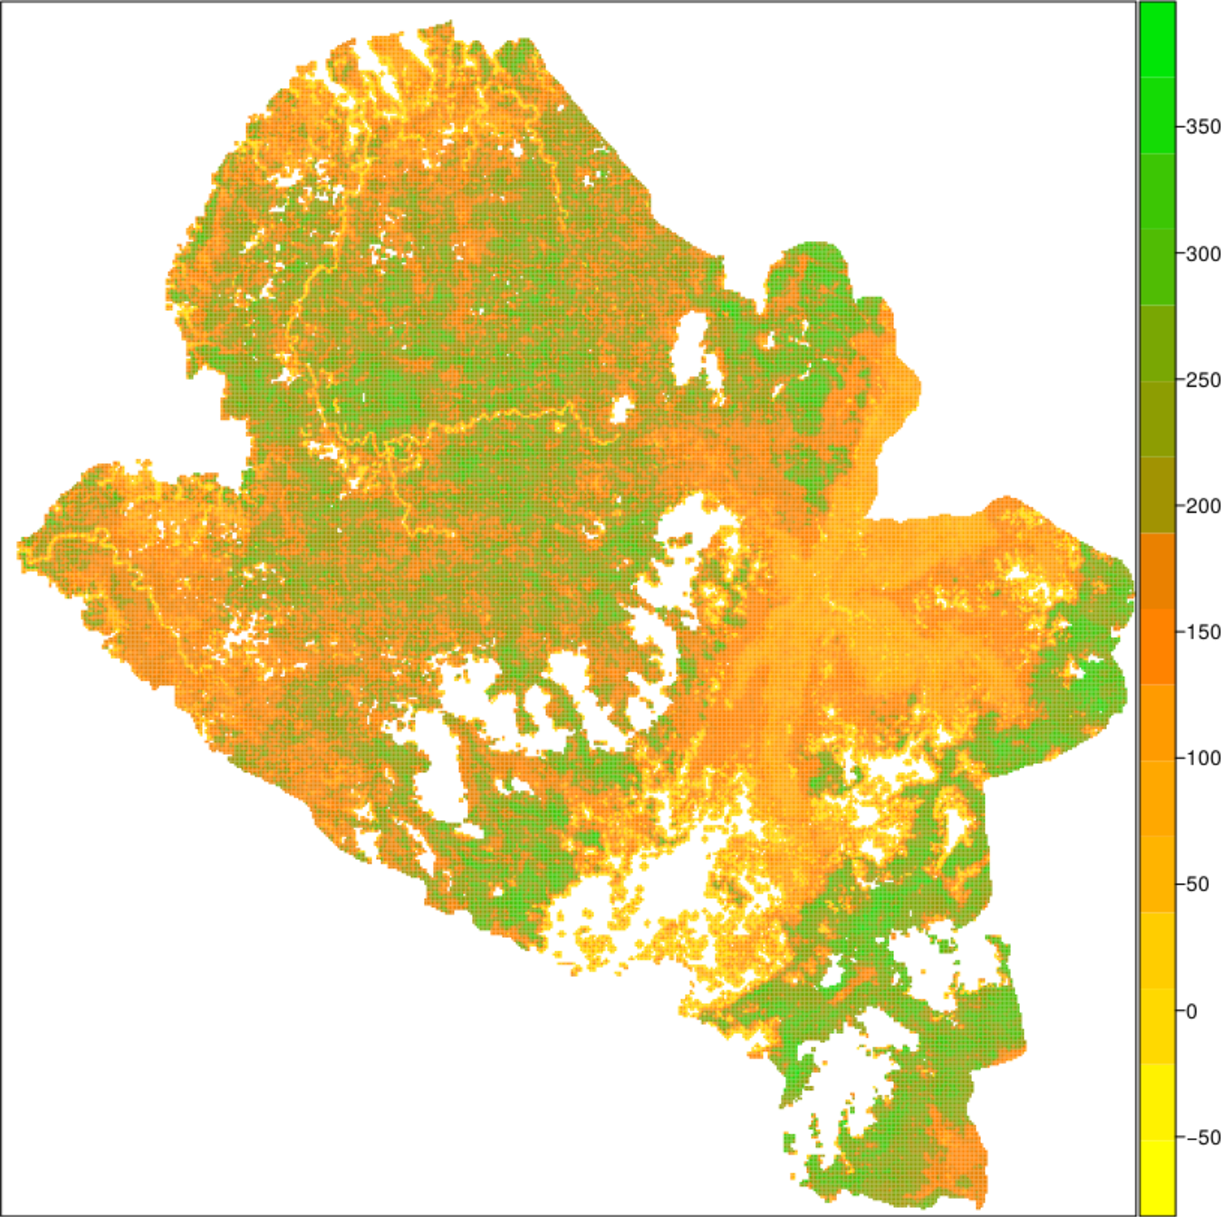
\includegraphics[width = 8cm]{mapaNarino.pdf}
  \caption{Department of Nariño biomass map years 2000-2003 \cite{baccini2008afirst}}
  \label{fig:mapaNarino}
\end{figure}

\subsection{Processing and data cleaning}

This research designs a data bse to capture data, as is shown in the figure~\ref{fig:landsatET}, la cual tiene 4 tablas. 

\begin{figure}
  \centering
  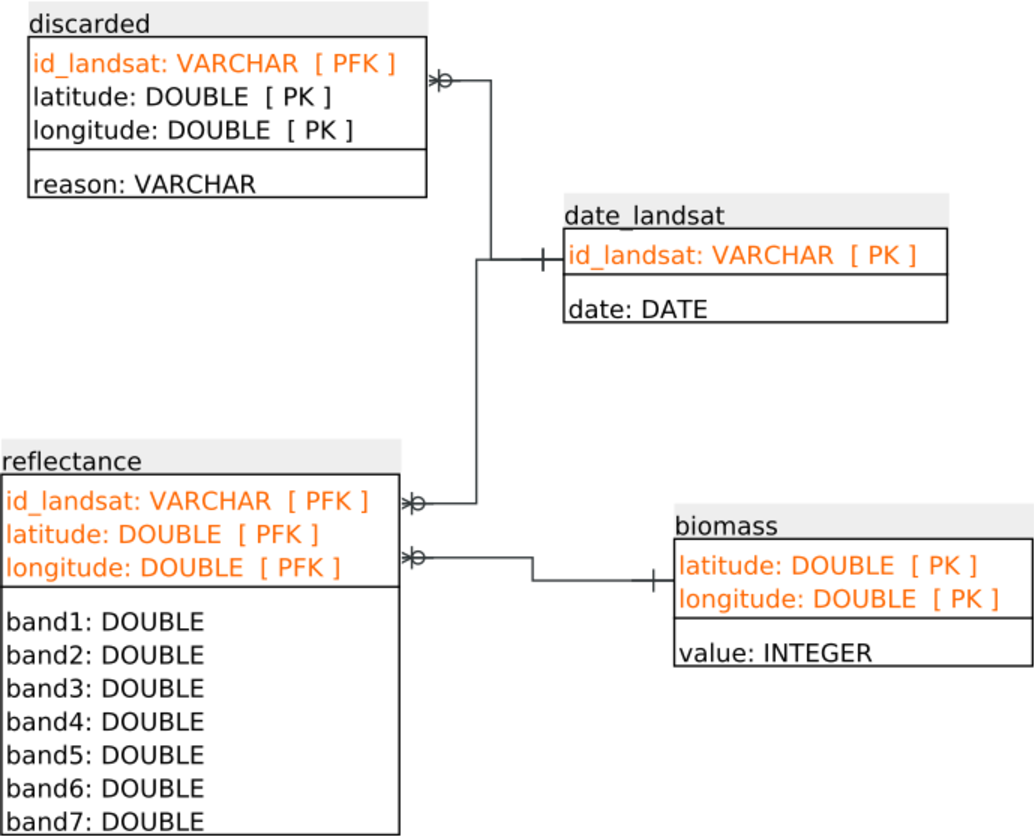
\includegraphics[width = 8cm]{landsatET.pdf}
  \caption{Landsat entity–relationship model}
  \label{fig:landsatET}
\end{figure}

Table date\_landsat: This table stores dates of each satellite image.

Table reflectance: This table stores data captured and converted in reflentance of the Landsat band (1 - 5,7) and temperature in kelvin scale of band number 6.

Table discarded: This table stores discarded data, by the next but not limited to: warm clouds, cold clouds, ambiguous data or not vegetation.

Table biomass: This table stores biomass map data from \cite{baccini2008afirst}.

To process the imagery and load the data base was written an script, this script capture the Digital Number of each satellite image and transform it in reflectance value. In this image processing, the script was complemented adding filters to detect warm clouds, cold clouds, ambiguous data as is show by the algorithm proposed by \cite{irish2000landsat}, in addition, the NVDI(normalized difference vegetation index) filter was apply to work with vegetation data only.

The table~\ref{tab:datos} shows the data obtained in this process.

\begin{table}
\caption{Data generated in process and data cleaning}
\label{tab:datos}
\centering
\scalebox{0.7}{
\begin{tabular}{c c c}
\toprule
 Name & Value& Detail\\
\midrule
Processed Landsat Images & 1321 & Department of Nariño images from years 2000 to 2014 \\
Total data & 51.076.512 & Total records form years 2000 to 2014 \\
Biomass data & 81.993 & Biomass records form years 2000 to 2003 by   \cite{baccini2008afirst}\\
Warm cloud & 3.731.768 & Records form years 2000 to 2014 \\
Cold cloud & 27.827.009 & Records form years 2000 to 2014 \\
No vegetation & 3.459.210 & Records form years 2000 to 2014 \\
Ambiguous & 11.987.340 & Records form years 2000 to 2014 \\
Reflectance valid data & 4.071.185 & Records form years 2000 to 2014 \\
\bottomrule
\end{tabular}}
\end{table}

\subsection{Regression analysis}

The regression analysis was performed using values from Landsat bands acquired from years 2000 and 2003, and biomas values obtained at \cite{baccini2008afirst}, to acquire a better model the Landsat bands values were grouped and the average of those were calculated to each point, by iterating with values no greater than N samples number, N from 1 to 45 samples, the best model obtained got at least 35 samples per point, this data set has 1009 records. The behavior of the others iterations shows that less quantity of samples generates more records and greater quantity of samples generates low quantity of records, both cases the result is a not good model.

In table~\ref{tab:metricas} is shown the results of metrics applied to analyzed models with 35 samples and 1009 data, which is the best model got by the research, this table was created using the open source library rminer presented by \cite{cortez2010data} to R tool.

\begin{table}
\caption{Metrics applied to analyzed models with 35 samples and 1009 data}
\label{tab:metricas}
\centering
\scalebox{0.7}{
\begin{tabular}{c c c c c c c}
\toprule
 & SAE & MAE & RAE & RMSE & COR & R2 \\
\midrule
ctree & 10406.58225 & 30.88007 & 65.04650 & 40.02893 & 0.69401 & 0.48165 \\
rpart & 10197.95826 & 30.26100 & 63.74249 & 39.37592 & 0.70520 & 0.49730 \\
kknn & 9147.51425 & 27.14396 & 57.17667 & 36.86581 & 0.74955 & 0.56182 \\
mlp & 9179.79310 & 27.23974 & 57.37843 & 34.70711 & 0.78122 & 0.61031 \\
mlpe & 8746.27740 & 25.95335 & 54.66874 & 34.57953 & 0.78309 & 0.61323 \\
ksvm & \textbf{8462.61487} & \textbf{25.11162} & \textbf{52.89570} & 34.67742 & \textbf{0.79830} & \textbf{0.63729} \\
randomForest & 8807.76477 & 26.13580 & 55.05306 & 34.70615 & 0.78239 & 0.61214 \\
mr & 10410.13919 & 30.89062 & 65.06873 & 38.61068 & 0.72000 & 0.51840 \\
mars & 8842.91866 & 26.24011 & 55.27279 & \textbf{33.96852} & 0.79161 & 0.62665 \\
cubist & 9012.54150 & 26.74345 & 56.33302 & 35.70576 & 0.77611 & 0.60235 \\
pcr & 10337.63121 & 30.67546 & 64.61552 & 38.59290 & 0.72023 & 0.51873 \\
plsr & 10337.63121 & 30.67546 & 64.61552 & 38.59290 & 0.72023 & 0.51873 \\
cppls & 10337.63121 & 30.67546 & 64.61552 & 38.59290 & 0.72023 & 0.51873 \\
\bottomrule
\end{tabular}}
\end{table}

Also, in this process was used the Boruta R package \cite{kursa2010feature}, this is a new features selection algorithm which found all relevant variables. The algorithm is designed as a wrapper to the random forest classification algorithm. The Boruta algorithm was used to establish if every Landsat bands used were relevant to find biomass, in figure ~\ref{fig:boruta} can be seen the relevance of Landsat bands to find biomass in the best model.

\begin{figure}
  \centering
  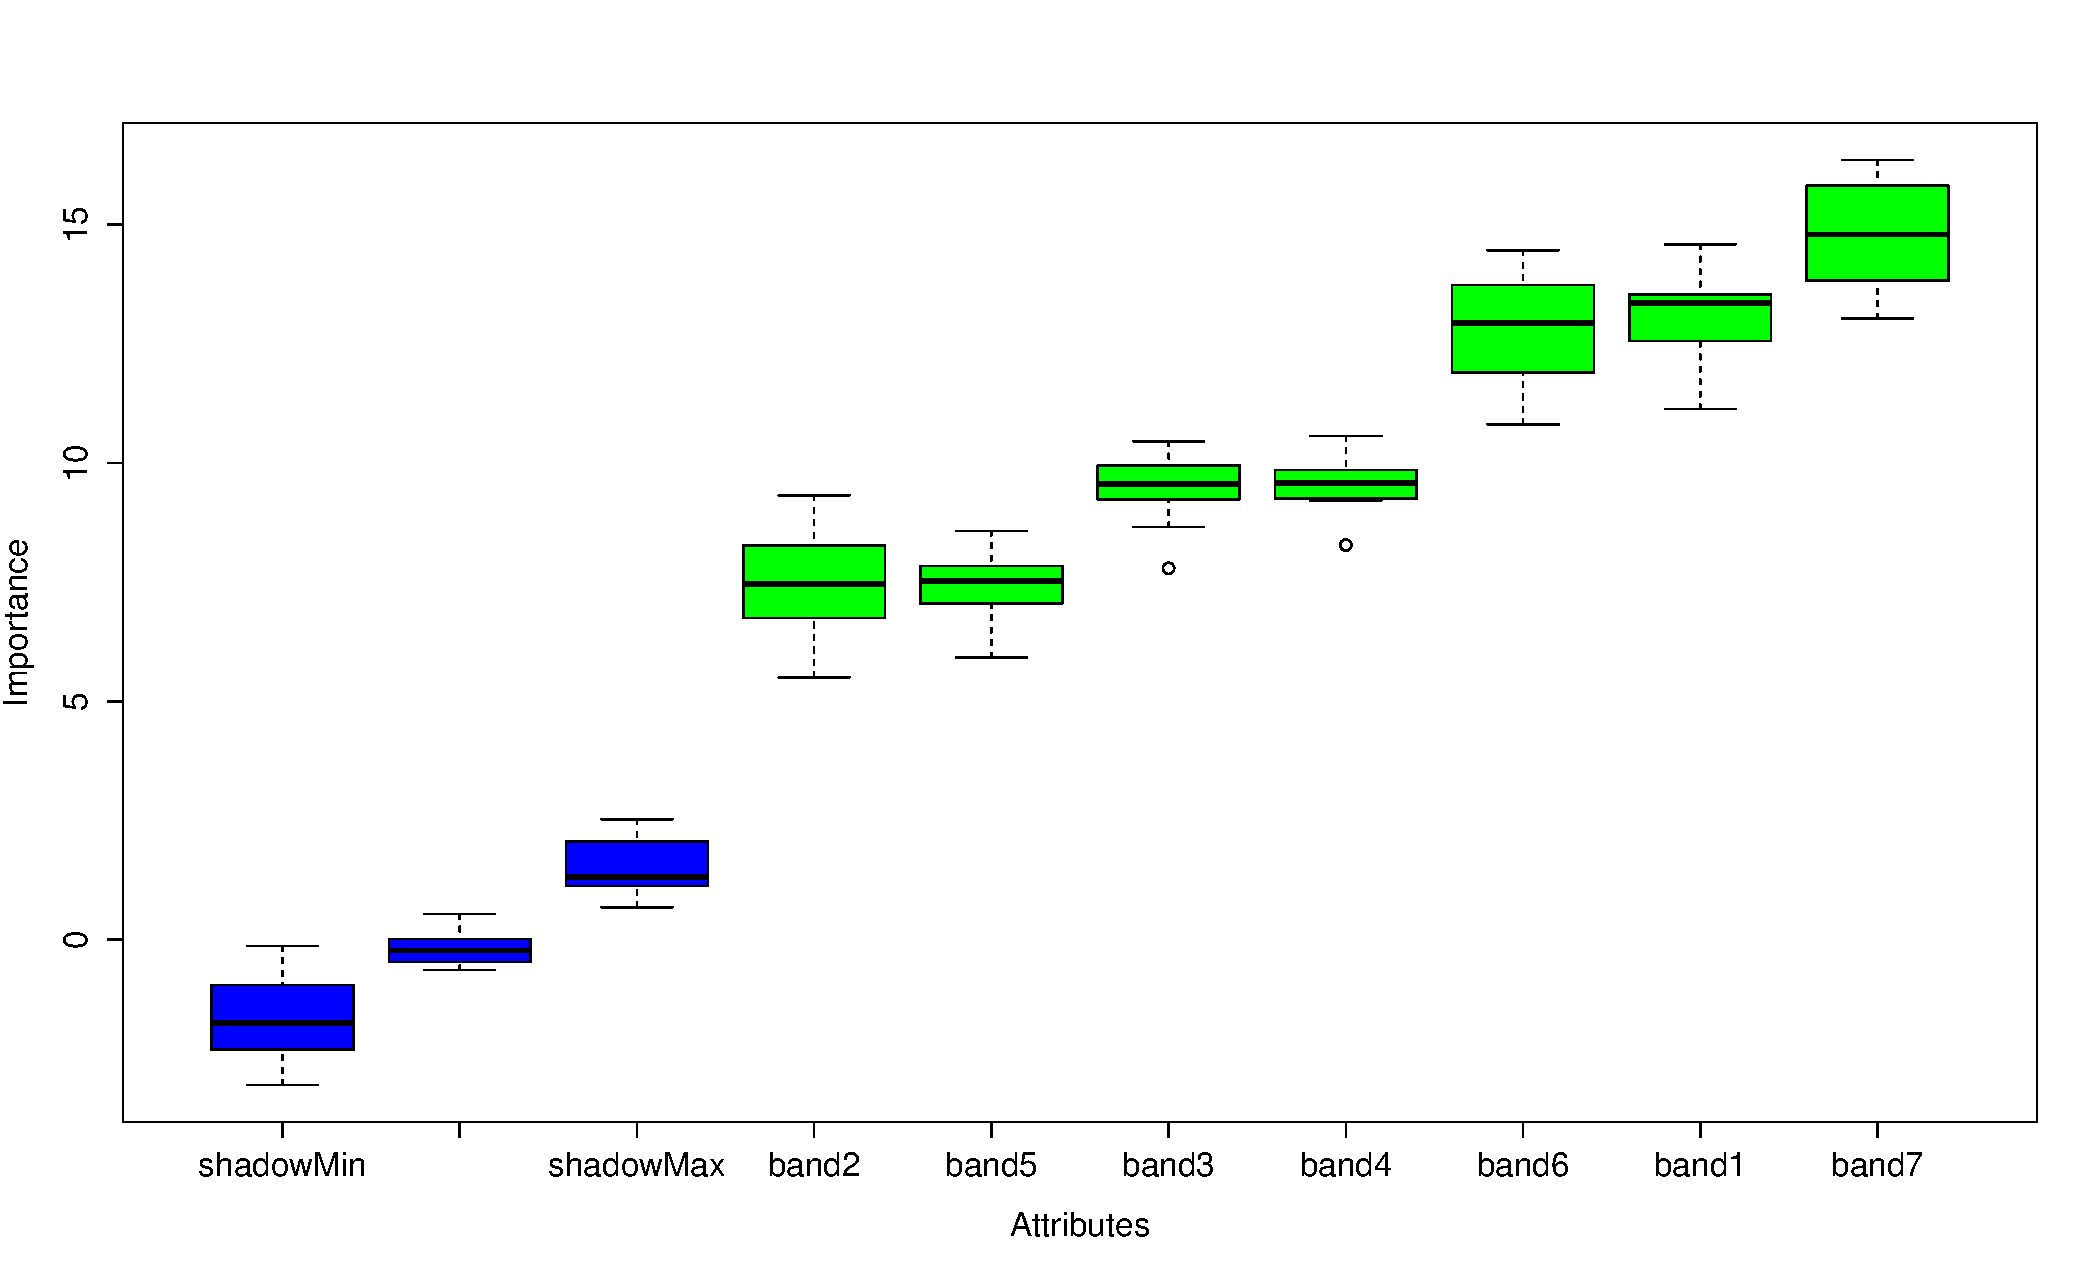
\includegraphics[width = 8cm]{boruta.pdf}
  \caption{Relevance of Landsat bands int regression analysis}
  \label{fig:boruta}
\end{figure}

\subsection{Maps construction}

To build the biomass maps were used Kriging method, this method provide a solution to the estimation problem based on a continuous model of stochastic spatial variation, the Kriging´s objective is estimate the value of a random variable, Z, in one or more points not sampled or over large blocks. 

The Kriging method has as input data from the sample, and a data matrix depending on the desired result image resolution, that is why the data samples were obtained applying the generated model in the regression analysis of grouped data by month, year and general in each point for years 2000 to 2014; and the data matrix was build with regular points with a 450 meters gap.
 
In figure ~\ref{fig:biomasaMes}, figure~\ref{fig:biomasaAnio}, and figure~\ref{fig:biomasaTotal}  is shown the monthly, yearly and general maps obtained for years 2000 a 2014 respectively. 
 
\begin{figure}
  \centering
  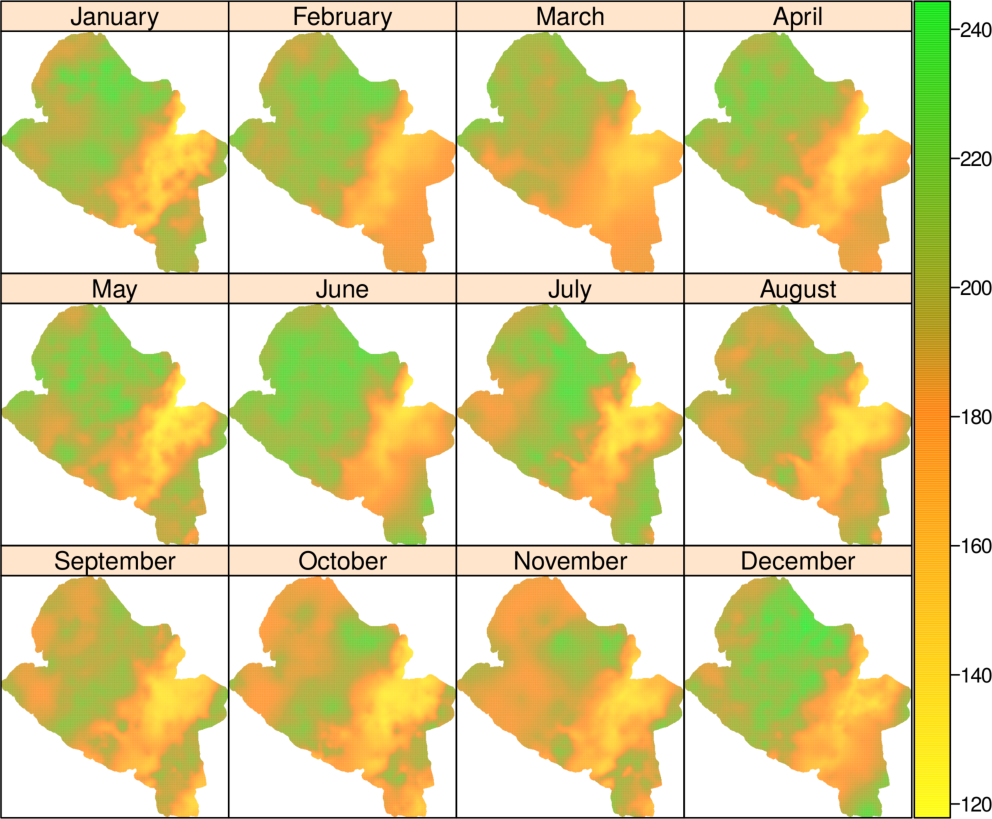
\includegraphics[width = 8cm]{mapMonthsBiomass.pdf}
  \caption{Monthly biomass maps}
  \label{fig:biomasaMes}
\end{figure}

\begin{figure}
  \centering
  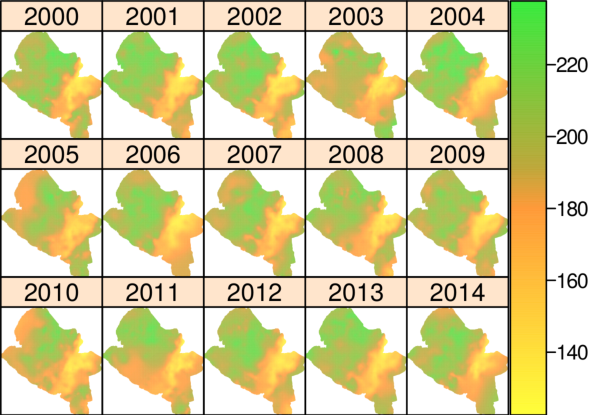
\includegraphics[width = 8cm]{mapYearsBiomass.pdf}
  \caption{Yearly biomass maps}
  \label{fig:biomasaAnio}
\end{figure}

\begin{figure}
  \centering
  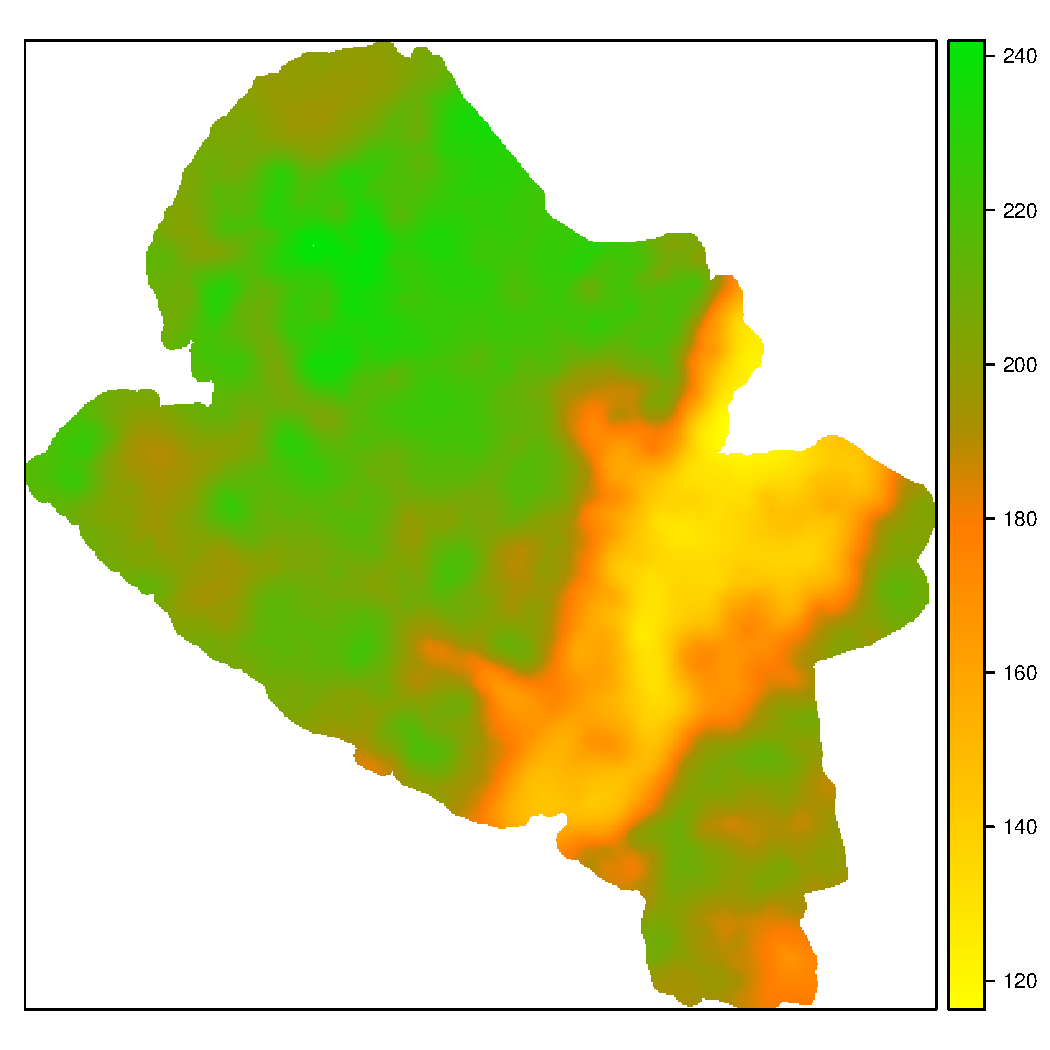
\includegraphics[width = 8cm]{mapGeneralBiomass.pdf}
  \caption{General biomass map years 2000-2014}
  \label{fig:biomasaTotal}
\end{figure}